\documentclass[11pt,letter]{article}
\usepackage[top=1.00in, bottom=1.0in, left=1.1in, right=1.1in]{geometry}
\renewcommand{\baselinestretch}{1.5}
\usepackage{graphicx}
\usepackage{natbib}
\usepackage{amsmath}
\usepackage{hyperref}

\def\labelitemi{--}
\begin{document}

\title{`A Fine Balance': Exploring the Interplay of Reproductive Strategies and Growth Dynamics in Trees}
\author{Xiaomao Wang} 
\date{\today}
\maketitle

\setlength{\parindent}{0pt}
\setlength{\parskip}{3pt}

%emw17Apr2025: I think your proposal is in good shape (yay!) except for the mathematical notation, so I will not review most of the text again. Thus, if you have any questions about changes or want me to verify that you entered them correctly, please highlight them in the PDF on the next round and I will check (also, if you change the text beyond the math notation, highlight it for me to check. 
% I would not include the new conceptual figures. I would be excited to discuss them with you but I think the proposal is too far along to add new figures like these now. We could add them if comments from your committee suggest we need them (and then we need to adapt the text or figures, as the two currently don't match enough). 
% Also, on the next draft can you confirm the counts in the seed trap figure are total seeds (sum of all stands for each species for each year)? 

\section{Introduction} 
The fundamental processes in a plant's life cycle—growth, reproduction, defense—all compete for the same resources. Plants must apply trade-offs to maximize their fitness when resources are limited. One of the most significant of these is the growth-reproduction trade-off, which is influenced by both environmental conditions and a plant's life history strategy \citep{grime1977evidence, stearns1998evolution}. In resource-rich environments, plants are able to allocate resources both to rapid growth and reproduction, while in resource-poor environments, plants often face a decision: they can either allocate resources to growth, ensuring their long-term survival, or they can invest in reproduction, which may come at the expense of growth \citep{bazzaz1997allocation}. This trade-off can lead to high variability in reproduction across years, which is manifested as mast seeding, an important reproductive strategy for many plant species \citep{pearse2016mechanisms}.\par

Mast seeding is the phenomenon of synchronized and variable seed production within plant populations. It determines regeneration within a population and is closely related to ecosystem-level functions that influence processes such as seed dispersal, predation and plant recruitment, since seeds can be food resources for many mammals or hosts for pathogens  \citep{davies2024seed, janzen1971seed, kelly1994evolutionary}. Mast seeding is widely observed in wind-pollinated tree species, but also occurs in \textit{Poaceae} as well as \textit{Diperocarpaceae} \citep{kelly2002mast}. Although there are several hypotheses explaining the potential mechanism selecting for mast seeding  \citep[e.g., predator satiation, resource matching, \textit{etc.}, discussed more in Chapter 2,][]{koenig2021brief}, the exact environmental factors that trigger it in different species and ecosystems are not fully understood. Current data suggest that it is mainly driven by specific climatic conditions that cause synchronized reproductive efforts of the species at population level  \citep{pearse2016mechanisms}. \par

Research on masting has often focused on its unique features, which makes it distinct from annual fluctuations in seed production of non-masting species---specifically its interannual variation, synchrony, temporal autocorrelation, and frequency \citep{hacket2021climate}. While annual fluctuations in seed production for non-masting species are generally more closely tied to short-term environmental factors (or may appear random), interannual variation in masting is not entirely random or caused by immediate environmental conditions; instead it should be synchronous across large spatial areas \citep[e.g., hundreds of kilometers,][]{kelly1994evolutionary}, and show distinct temporal autocorrelation, where a mast year is typically followed by several years of low or no seed production. Finally, mast years often occur at a certain frequency, with some species exhibiting a more fixed interval (e.g., every 2-3 years) and others a more irregular pattern (e.g., 2-5 years). \par

Masting plays an important ecological role by influencing seed dynamics and broader ecosystem processes. According to the predator satiation hypothesis, mast years overwhelm seed predators by producing abundant seeds, ensuring that some seeds will survive and germinate. In this way, plants can regulate predator populations and enhance seedling establishment. Mast seeding also contributes to the creation of seed banks, which provide a reserve of seeds that help the population buffer against environmental variability, allowing seeds to wait for favorable conditions to germinate \citep{venable1989modeling}. This strategy not only improves seedling survival in the short term but also promotes long-term regeneration, helping to maintain a plant population over time.\par

Ongoing anthropogenic climate change is extending growing seasons, shifting precipitation patterns, and likely making environmental variability less predictable. These changes may influence the balance of the growth-reproduction trade-off through altered plant resource availability and consequently, masting behavior, which will not only affect the forest population dynamics itself, but also the seed predator community that relies on the forests. Understanding how these dynamics function, and the role that climate plays, is critical for predicting future forest composition and regeneration, but the complexity of masting has slowed progress. Currently, we lack a comprehensive model to predict how climate change will affect masting that includes the relationship between growth and reproduction, and can make predictions across different species and ecosystems.\par

The aim of my thesis is to investigate how masting as a reproductive strategy, is related to the growth dynamics of tree species and their role in forest ecosystems, particularly in the context of climate change. Using Mount Rainier as a case study, my proposed research will address three key questions: (1) Which reproductive traits are associated with masting? Addressing this will help to potentially identify what triggers masting across species, and in different environments. (2) Is there a detectable trade-off between mast seeding events and tree growth? (3) How will changing climate conditions affect seed dynamics at Mount Rainier? Answering these questions will contribute to our understanding of how masting shapes the growth and regeneration dynamics of coniferous forests in Mount Rainier, with inference on how masting dynamics might be related to growth and environmental changes in other coniferous forests globally.\par

\section{Explore which reproductive traits are relevant to masting}
Masting is widely observed across different plant lineages in different biomes, with several major hypotheses for how masting could yield fitness benefits, compared to reproducing every year \citep{koenig2021brief, waller1979models}. The most commonly accepted hypothesis for masting is the predator satiation hypothesis, which suggests that masting overwhelms seed predators with a large seed crop in one year, then starves these predators during the following years with a low seed crop \citep{janzen1971seed}. By manipulating the seed predator population, masting should thus increase the likelihood of seed survival and germination. Another widely accepted hypothesis focuses on the benefits of masting for pollination success---the pollination coupling hypothesis \citep{crone2014resource}. Under this hypothesis, highly synchronized flowering improves pollination success and results in more seeds. While both of these hypothesis focus on reproductive success, the resource matching hypothesis focuses more on resources constraints. Its suggests that a fixed fraction of resources is allocated to reproduction every year \citep{kelly1994evolutionary}. In years when environmental conditions are favorable, plants accumulate more resources, which allows them to produce a larger seed crop during a masting event. Under this hypothesis, masting is not driven by a selective advantage per se, but rather a result of resource availability constraint, with the potential for increased reproductive output when resources are abundant. Thus, masting may appear as a neutral or incidental outcome of environmental conditions rather than an adaptive strategy to increase fitness. Closely related to this is the environmental cues hypothesis, which suggests that certain environmental events trigger masting \citep{pearse2016mechanisms}. These hypotheses are not mutually exclusive and may hold true for different species in different environments.\par

Based on these hypotheses, we can link specific traits to the phenomenon of masting. Since masting is a reproductive event, the most relevant traits are likely related to seed reproduction, which occurs through at least three critical stages: pollination, seed maturation and seed dispersal \citep{satake2021studying}. Each stage presents unique opportunities that can influence the overall success of mast seeding. During pollination, traits can be linked to the pollination coupling hypothesis, which suggests that synchronized flowering improves pollination success and then seed production, such as whether a plant is monoecious or dioecious. Because monoecious plants may have higher pollination success, compared to dioecious plants  \citep[where separate genders for each individual plant may reduce pollination success in low-density populations,][]{bawa1980evolution} we predict that monoecious plants, by ensuring higher fertilization success, may be more likely to mast. Another important trait is duration of flowering, since a longer flowering period might increase pollination success \citep{knight2005pollen}, thus increasing seed set. Masting species are also most likely to be wind-pollinated, so pollination is not restricted by the number of pollinators when large numbers of flowers bloom simultaneously \citep{bogdziewicz2017masting, bogdziewicz2020flowering}.\par

After pollination, fertilized seeds enter the maturation stage, which is more related to the resource matching hypothesis. Traits such as leaf longevity and determinacy, which influence the timing of seed development and a plant's ability to invest in reproduction, are thus likely important at this stage. Determinacy \citep[whether the leaf material is prebuilt the year before or not,][]{lechowicz1984temperate} may influence how quickly plants can shift their resource allocation into reproduction. Plants with determinate growth---because they have prebuilt and thus `ready' buds---may be able to shift resources more rapidly toward reproduction, potentially leading to higher reproductive output in a favorable year. In contrast, indeterminate growth could be slower to respond since new bud tissues need to be built, which could result in more prolonged resource allocation to other growth functions, possibly reducing the ability to invest heavily in a single reproductive event like masting.  Our understanding of determinacy across species, however, is still poor \citep{halle1978architectural, kozlowski1966shoot, marks1975relation} and thus an alternative prediction is also possible, where plants with determinate buds must invest too far in advance to shift enough in response to favorable years, while indeterminate species can rapidly develop new buds and thus shift resources quickly to reproduction.  Leaf longevity could also play a role in addition to determinacy. As greater longevity facilitates more carbon fixation and thus could enhance the resources available for reproduction \citep{adler2014functional}, species with greater longevity may more easily build up resources for seed production and thus be more like to mast.\par  %emw17Apr2025: some edits to end of paragraph

When seeds mature and are ready for dispersal, the role of seed predators becomes crucial. According to the predator satiation hypothesis, plants can manipulate the population of seed predators by producing large numbers of seeds in masting year and low number so f seeds in following years. Masting species, however, may also rely on seed dispersers to carry seeds away from the parent tree, increasing the chances of seedling survival \citep{janzen1971seed, silvertown1980evolutionary}. In this context, seed traits such as seed size, nutrient content, dispersal mode, seed dormancy and seed longevity all can play important roles. Larger seeds with higher nutrient content might be more attractive to seed predators, so they are more likely to benefit from masting events. Seed dormancy and seed longevity help ensure that seeds do not germinate immediately after dispersal, allowing them to wait for better conditions to establish in a more favorable environment since mast events only occur once every few years.\par

My proposed work advances on previous studies in this areas, which have explored the relationship between limited traits with interannual variability in seed production to test for support for different hypotheses \citep{fernandez2019nutrient, journe2023evolution, pearse2020biogeography}, but did not explain how different environmental conditions may link to which reproductive traits are more critical. In this meta-analysis, I will include more reproductive traits associated with different hypotheses to investigate how these traits are related to a species' tendency to mast in different forest types and biomes.\par

\subsection{Research Question and Objectives}
Which seed traits are related to masting? Additionally, do these traits relate to different masting hypotheses vary by species or environment?
	\begin{itemize}
	\item \textbf{Investigate trait associations:} Analyze the relationships between specific reproductive traits and masting event and frequency to determine which traits are more important in masting for different species.
	\item \textbf{Compare across different environments:} Compare the most critical traits across different forest types and biomes to determine if they vary.
	\end{itemize}
\subsection{Methods}
This chapter aims to explore the relationship between reproductive traits and the tendency of a species to mast in different environments through a meta-analysis.\par %emw17Apr2025: be careful when using 'various' -- it stresses a bit of 'this or that' similar to 'miscellaneous' and is not a good synonym for different
\textbf{Data collection}\\
Data for this meta-analysis will be primarily sourced from following resources:
	\begin{itemize}
	\item \textbf{Silvics of North America:} Provides a comprehensive database of tree species and their reproductive characteristics in North America, will be our main dataset. It includes flowering traits, seed dispersal traits, mast cycles and forest types. For biomes, I will use the information in the distributional map provided by the book and categorized into temperate, subtropical and tropical. For forest type, I will extract information from the section of associated forest cover, and try to categorize it according to North American forest cover types.
	\item \textbf{MASTREE+:} This is a specialized database focused on tree species' mast seeding behavior, which will be a supplemental source for identifying species tendencies for mast seeding and interannual variability.
	\item \textbf{Co-mast:} This is a specific database on harmonized seed production data for woody plants across US, which will also be a supplemental source for mast cycle.
	\item \textbf{Kew Seed Dataset, Worldwide Seed Mass Dataset, USDA Seed Manual:} These sources will offer supplementary information on seed mass and other reproductive traits.
	\end{itemize}
\textbf{Statistical Analysis and Model Development}\\
The main analysis will involve logistic regression to determine the likelihood of mast seeding based on the selected reproductive traits and environmental variables. The response variables, whether a species masts or not and the coefficient of variation (CV) of the mean annual seed crop,  which is widely used in masting related research to describe the highly variable year-to-year production of seeds, will be analyzed separately to evaluate the occurrence and variability of mast seeding behavior \citep{kelly2002mast}.

\subsection{Significance} 
Studying the reproductive traits related to masting can provide valuable insights into reproductive strategies and the broader ecological impacts on forest ecosystems. First, it can help explain the potential mechanisms that drive this complex reproductive strategy, shedding light on why certain species mast while others do not in different environments. Examining traits such as seed size, nutrient content, dormancy, and longevity can yield insights into how these characteristics influence the success of seed production and dispersal during mast years, which may then relate to seed predators' population dynamics.\par

Additionally, understanding these relationships can help us to predict how environmental factors, such as climate change, may impact masting behavior in the future. For example, knowing which seed traits are most relevant to masting behavior in specific ecological contexts can help us anticipate how shifts in temperature, precipitation, and other environmental cues might change masting patterns. By addressing the question of what causes masting by looking at seed traits, we may better understand the dynamics of forest ecosystems.\par

\section{Understanding the relationship between masting and growth}
The growth-reproduction trade-off suggests that increased investment in one process often comes at the expense of the other \citep{grime1977evidence, stearns1998evolution}. For trees, the decision to allocate resources to a large seed crop during a masting year can significantly affect overall growth dynamics \citep{hacket2016tree}. This relationship between growth and reproduction can be complex, as the years leading up to a masting event may involve resource accumulation for reproductive efforts, while the years following masting could exhibit a different pattern, influenced by less demand for reproduction \citep{kelly1994evolutionary}.\par

With anthropogenic climate change, tree growth in generally expected to increase, as warmer temperatures increase growth rates and provide trees with more time to growth each year with extended growing season \citep{keenan2014net, finzi2020carbon}. Most climate models predict a positive relationship between temperature and growth \citep{friedlingstein2022global, ito2020global}. However, recent studies have questioned whether the extending of growing seasons due to warming has actually led to increased tree growth \citep{dow2022warm, green2022limits}. Studies have suggested that biotic factors, such as intrinsic species differences, how plants allocate the additional carbon gained during warmer seasons, also play a significant role \citep{hacket2016consistent}. In the context of masting, these dynamics become even more complex, underscoring the importance of understanding how different tree species will behave in future climates.\par

%emw17Apr2025: below 'various' sounds fine (it sounds like: they look at some climate factors, which ones is not important) 
While many studies have examined how climate influences both growth and reproduction, often comparing responses to various climate factors \citep{bajocco2021characterizing, koenig2020can, redmond2019resource, sanchez2011trade}, only a few have directly investigated the growth-reproduction trade-off in the context of masting. The majority of these studies have focused on oak and pine species. Studies on pines have emphasized on the allocation to defence, rather than looking at trade-off between growth and reproduction specifically \citep{larrinaga2024resource, redmond2019resource}. Research on oaks found little evidence of a strong, consistent trade-off between radial growth and seed production \citep{koenig2020can, patterson2023acorn}. However, this lack of evidence may be due to a  large biomass allocation to roots, as oaks generally have deep root systems and tend to allocate more resources to root development from youth to maturity \citep{burns1990silvics}. In contrast, the species I will use in this study, either have shallow roots or do not develop resources-expansive taproots, thus they may exhibit a different response.\par

The relationship between masting and growth could also differ across elevations, where resource availability and environmental stresses vary. Trees at higher elevations may experience a more pronounced trade-off between growth and reproduction due to increased resource limitation and harsher environmental conditions (Figure. \ref{fig:conceptual2}). By examining different species at varying elevations, we can gain a better understanding of the potentially complex relationship among resources, growth, and reproduction.\par

Combining Mount Rainier's unique elevational gradient with long-term tree growth data from tree rings, this chapter explores the relationships between resource availability, growth and reproduction in six common coniferous species. It emphasizes how the strength of trade-offs that shape reproductive strategies may differ across varying ecological conditions.
\subsection{Research Question and Objectives}
Is there a detectable trade-off between mast seeding events and growth?
	\begin{itemize}
	\item \textbf{Assess Growth Patterns:} Test for a trade-off by analyzing historical annual growth of selected tree species in relation to their masting events.
	%emw17Apr2025: below 'various' does not work, also you should keep info related to species together (species with different allocation strategies, then elevation, not: species, elevation, allocation strategies) 
	\item \textbf{Compare Species Responses:} Evaluate the differences in masting and growth responses among six tree species with different resource allocation strategies across different elevations.
	\end{itemize}
\subsection{Methods}
This chapter aims to examine the growth-reproduction trade-off in relation to mast seeding for six common conifer species at Mount Rainier across different elevations. To explore this relationship, I will incorporate long-term seed trap data with historical growth data derived from tree core samples, and use statistical approaches to analyze their relationship.\par

\textbf{Study site and sample collection}\\
I will conduct this study in Mount Rainier National Park, Washington, USA. I will focus on six common conifer species that exhibit varying masting behaviors and occur across different elevations in the park (Figure. \ref{fig:sites}). The data I plan to use in this chapter include two components:	
\begin{itemize}
	\item \textbf{Long-term seed data:} Our collaborator Dr. Janneke Hille Ris Lambers, has been collecting stand-level seed production data using seed traps since 2008, which will provide a valuable record of masting events across different stands and elevations at Mount Rainier  (Figure. \ref{fig:seed}).
	\item \textbf{Tree growth data:}  To assess the historical growth of individual trees, I will collect cores from targeted species in Table. \ref{table:species} in each stand with long-term seed data. Within each stand, there are at least two targeted species, and each species appears in at least four stands. I plan to collect tree cores from 25 individuals per species per stand, covering a size gradient. To make sure the trees we core are mature enough to reproduce at least 10 years ago to match with seed trap time window, I will only collect from trees with DBH greater than 25 cm. Additionally, I will prioritize individuals that are close to seed traps to better correlate with seed data. I will core trees at breast height using increment borers, taking two tree cores from the opposite sides of the tree while avoiding slopes. To account for at least 15 years of growth and for cross-dating purposes, I will collect long cores of 25 cm from larger trees with a DBH above 50 cm, while for smaller trees, I will core to the center if possible.
	\end{itemize}
\textbf{Tree core processing}\\
I will prepare the cores for analysis by sanding them with fine grit sandpaper (up to 2000 grit depending on the visibility of rings) to ensure a smooth, clear surface. For cores with rings that are difficult to distinguish, I will use a microtome to further enhance the visibility of the rings, creating a clear surface for better quality.\par

After preparation, I will scan the cores using a high-resolution camera to capture detailed images of the growth rings, then I will analyze the images with CooRecorder, a software used to measure tree ring width. I will also double check the cross-dating results with COFECHA, a computer program that assesses the quality of crossdating and measurement accuracy of tree-ring series \citep{cook2013methods, speer2010fundamentals}.\par

\textbf{Statistical analysis}\\
My proposed model investigates the trade-offs between growth (radial growth) and reproduction (seed production). It partially pools species and stands to allow for variation, while sharing information between groups to produce an overall estimate.\par

%emw17Apr2025: I suggest you pull out the math you have here into a new tex file and work on it separately from the proposal (I suggested this before, and I am suggesting it again). Then we can work on the model. Trying to decide on the model here within the proposal is not easy for me. If you want to keep doing it, you can, but it will take a while I believe to correct all of it enough to send the proposal to your committee. So I recommend you proceed on two tracks (1) pull out the math you have here into a new tex file and work on it separately from the proposal with me and with Victor, (2) keep your seed model here then in text only describe your progress towards the next steps of the model (example shown below that builds on text below).  
% My proposed model investigates the trade-offs between growth (radial growth) and reproduction (seed production). It partially pools species and stands to allow for variation, while sharing information between groups to produce an overall estimate. Thus far, I have developed the model for seed production (below) and am developing the model for radial growth, which is more complex in that I need to decide how to remove size effects for each tree, then scale up all trees to a stand-level estimate that I can then use to model the relationship between growth and reproduction. 
\textbf{Likelihood for Seed Production}\\

The seed count for a particular stand \(j\), species \(sp\), and year \(y\) follows a negative binomial distribution with mean \(\lambda_{j,sp,y}\) and dispersion term \(\phi\):

\[
\text{Seed}_{j,sp,y} \sim \text{NegBinomial}(\lambda_{j,sp,y}, \phi)
\]

The modeled seed count (\(\lambda_{j,sp,y}\)) for stand \(j\), species \(sp\), and year \(y\) is:

\[
\log(\lambda_{j, sp, y}) =\alpha_{\text{0,seed}} + \alpha_{\text{sp}} + \alpha_{\text{j}} + \beta_{\text{1,sp}} \cdot \text{Growth}_{j,sp,y} + \beta_{\text{2,sp}} \cdot \text{Growth}_{j,sp,y-1} + \beta_{\text{3,sp}} \cdot \text{Elevation}_{j}
\]

Where:\\
\(\alpha_{\text{0,seed}}\) is the grand mean across all species, stands and years;\\
\(\alpha_{\text{sp}}\) is the species-specific intercept for species sp;\\
\(\alpha_{\text{j}}\) is the stand-specific intercept for stand j;\\
\(\beta_{\text{1,sp}}\) is the slope for the relationship between current-year growth and seed production for species \(sp\);\\
\(\beta_{\text{2,sp}}\) is the slope for the relationship between previous-year growth and seed production as the lag effect for species \(sp\);\\
\(\beta_{\text{3,sp}}\) is the effect of elevation on seed production for species \(sp\).\\


\textbf{Likelihood for Radial Growth}

The log of the radial growth \(\text{Growth}_y\) of individual tree \(i\) for a particular stand \(j\), species \(sp\), and year \(y\) follows a normal distribution with mean\(\mu_{i, y_{\text{sp}, j}}\) and standard deviation \(\sigma_{\text{growth}}\):

\[
\log(\text{Growth}_i) \sim \text{Normal}(\mu_i, \sigma_{\text{growth}})
\]

Where the mean \(\mu_i\) is:

\[
\mu_i = \alpha_{\text{0,growth}} + \alpha_{\text{sp}[i]} + \alpha_{j[i]} + \beta^{\text{sp}[i]}_1 \cdot \text{Elevation}_{j[i]}
\]

Where:\\
\(\alpha_{\text{0,growth}}\) is the grand mean across all species, stands and years;\\
\(\alpha_{\text{sp}[i]}\) is the species-specific intercept for species sp;\\
\(\alpha_{j[i]}\) is the stand-specific intercept for stand j;\\
\(\beta^{\text{sp}[i]}_1\) is the slope for the relationship between elevation and growth for species \(sp\).\\

\subsection{Significance}
Understanding the relationship between masting and growth is important for predicting how tree species will respond to changing environmental factors, particularly in the context of extended growing seasons with climate change, where how trees allocate additional carbon can impact the global carbon cycle. By examining how these processes interact, we can gain insights into the adaptive strategies of different species and their potential resilience or vulnerability to future climate changes. This knowledge could help us make more informed predictions about future forest dynamics, including shifts in species composition, regeneration, and ecosystem health. As climate conditions continue to shift, understanding the  masting behavior and growth responses will be essential for effective forest management and conservation efforts, helping us to anticipate changes and make management plans that will support the sustainability and resilience of forest ecosystems.\par

\section{Investigate how changing climate affect masting dynamics}
Plants need to assimilate enough resources to produce seeds, a process that requires a combination of environmental conditions such as light, water, nutrients and suitable temperature. These factors directly influence mast seeding by affecting seed development process or affect it indirectly through their effects on flowering and growth. Flowering, for instance, is regulated by daylength, with light influencing the production of hormones that control both flowering and growth \citep{lau2010plant}. Light is also crucial for photosynthesis, which supports healthy plant growth. Water is another essential element for both flowering and fruiting. When water is limited, plants conserve energy, leading to fewer or smaller flowers, reduced pollination, or early flower shedding. After fertilization, water continues to play an important role in the expansion and maturation of seeds. Beside its direct effects on reproduction, water stress also inhibits growth, limiting the resources available for reproduction \citep{hsiao1973plant, anjum2011morphological}. Nutrients, both macronutrients and micronutrients, are essential for both energy transfer and storage, playing a significant role in the formation of flowers and seed development. Nutrient availability influences the timing of flowering and seed formation, with well-nourished plants more likely to flower at the appropriate time and set seeds successfully. Temperature, especially spring temperature, is one of the most widely studied climatic factors linked to masting events \citep{bajocco2021characterizing, moreira2015effects, schauber2002masting, bogdziewicz2024evolutionary}, as it plays a critical role in successful pollination and seed development.\par

Exploring the relationship between environmental factors and mast seeding behavior can help us to understand how climate change may impact masting events. The four main features of masting: interannual variation, synchrony, temporal autocorrelation, and frequency are all likely to be affected by climate change in different ways \citep{hacket2021climate}. Climate change is also expected to extend the growing season, allowing trees to allocate more carbon to growth and reproduction \citep{keenan2014net}. Additionally, warmer temperatures could increase the frequency of droughts, which would limit water supply. In areas with year-round snow cover, temperature changes may also alter water dynamics, affecting the timing and availability of water, which is critical for tree growth and reproduction. These shifts could have profound implications for the frequency and intensity of masting events.\par

Another important factor in the flowering and fruiting process is environmental `vetoes', which occur when weather events or environmental conditions prevent plant processes, even when resources are adequate \citep{bogdziewicz2022will}. Environmental vetoes can take two forms: (1) a lack of weather cues, such as when specific weather conditions required to trigger flowering or fruit maturation are not met, preventing reproduction despite adequate resources; and (2) extreme weather events, such as frost, drought, or heavy rainfall, which can directly damage plant tissues, including shoots, flowers and fruits, thereby preventing successful reproduction. With climate change, environmental vetoes may become more frequent, which is generally considered detrimental to plants. However, studies have shown that environmental vetoes preventing seed production in certain years can actually facilitate masting, allowing for higher regeneration success \citep{bogdziewicz2018correlated, bogdziewicz2019environmental}. Therefore, understanding how environmental vetoes influence seed production in different species and regions is critical for predicting future forest dynamics.  Once we understand how various environmental factors influence different aspects of masting, we can make better predictions of masting events and thus have a better understanding of how future changing climate may shape the seed dynamics in this region \citep{hacket2021climate}.\par

Elevation has long been used as a proxy for climate change in ecological studies, since it is closely linked to a variety of climatic factors, particularly temperature and water availability \citep{korner2007use}. It provides a natural system to study the long-term, large-scale effects of climate change on communities and ecosystems which cannot be accomplished by experiments \citep{sundqvist2013community}. By using elevation as a proxy for climate change, we can better understand how plant populations at different elevations respond to environmental factors and refine predictive models that incorporate shifting climatic variables at finer spatial resolutions. This approach also helps us understand vegetation shifts in ecosystem within a region.\par

Mount Rainier provides an ideal location for studying how climate change may impact forest dynamics, as it features a distinct elevation gradient and diverse snowmelt patterns. The rain shadow effect on different sides of the mountain also creates varying water availability. The climate in this region has already undergone significant changes in recent decades and, by combining historical seed data with climate data, we can explore the relationship between climatic variables and various aspects of mast seeding.\par

This chapter aims to understand how masting patterns are influenced by environmental factors. By investigating the large variance in interannual masting patterns, and exploring the relationship between spatial as well as temporal changes in masting across elevational gradients, we can better understand how climate change will impact seed dynamics in this area.\par

\subsection{Research Question and Objectives}
How does changing climate affect seed dynamics at Mount Rainier?
\begin{itemize}
\item\textbf{Identify Environmental Influences:} Investigate how key environmental factors (e.g., temperature, precipitation) are related to masting events at Mount Rainier.
\item\textbf{Climate change proxy:} Use the elevational gradient at Mount Rainier as a proxy for changing climate conditions to compare how masting behavior varies across different elevations.
\item\textbf{Develop Predictive Models:} Develop predictive models of masting behavior across elevations to forecast future seed dynamics under changing climate conditions.
\end{itemize}
\subsection{Methods}
This chapter aims to investigate how climate change influences seed dynamics at Mount Rainier, focusing on the relationship between mast seeding patterns adapted to local climatic conditions across different elevations for the same species. By using long-term seed trap data and corresponding climate data, I will assess how seed production synchrony and variability change along the elevation, which is used as a proxy for climate change for the same species we used in last chapter.\\
\textbf{Data collection}\\
\begin{itemize}
\item\textbf{Long-term seed data:} The same long-term seed trap data from last chapter.
\item\textbf{Local climate data:}  Our collaborator Dr. Janneke Hille Ris Lambers has data logger in the stands recording long-term soil moisture, ambient temperature and light data.
\end{itemize}
\textbf{Statistical Analysis and Model Development}\\
\begin{itemize}
\item\textbf{Time series model, mixed-effect models:}I will build upon the model developed in Chapter 2, which explores the growth-reproduction trade-off during mast seeding events, to create a more climate-sensitive model of mast seeding dynamics. This extended model will incorporate climate variables such as temperature and precipitation to assess how changing climatic conditions may alter the frequency, magnitude, and synchrony of mast seeding events. \\
\item\textbf{Predictive modeling:} I will develop predictive models to forecast future trends in masting behaviours at Mount Rainier under projected climate scenarios. These models will use climate projections for this region to predict how seed dynamics might shift in response to future climate change.
\end{itemize}
\subsection{Significance}
Changes in masting behavior can have cascading effects on forest dynamics, including seed predator interactions and the regeneration success of tree species. Since masting events can provide a large food source drives population dynamics of lots of mammals in the forest, changes of masting patterns will alter these ecological relationships, and the overall structure of ecosystems. Fore example, if climate change causes masting events to be less synchronized across species or elevations, it will affect seed availability for animals that rely on them as food source, potentially impacting their survival and reproduction.\par

Masting will also affect the regeneration of tree species itself. Many tree species rely on mast seeding years to establish successful new seedlings in the face of competition and predation. If climate change affects the frequency or intensity of mast seeding events, the successful regeneration of some tree species might be affected. Thus, understanding how these characteristics of masting might be influenced by climate change is essential for predicting the resilience of forest ecosystems.


\bibliographystyle{besjournals}
\bibliography{Proposal} 
\begin{table}[htb]
	\centering
	\small
	\caption{Targeted species}
\begin{tabular}{|p{5cm}|p{5cm}|p{5cm}|}
\hline
 Tree species & Common name\\ \hline 
\textit{Abies amabilis} & Pacific silver fir \\ \hline
\textit{Pseudotsuga menziesii} & Douglas fir\\ \hline
\textit{Tsuga heterophylla} & Western hemlock\\ \hline
\textit{Tsuga mertensiana} & Mountain hemlock\\ \hline
\textit{Thuja plicata} & Western redcedar\\ \hline
\textit{Callitropsis nootkatensis} & Yellow cedar\\ \hline
\end{tabular}
\label{table:species}
\end{table}

\begin{figure}[htb]
	\centering
	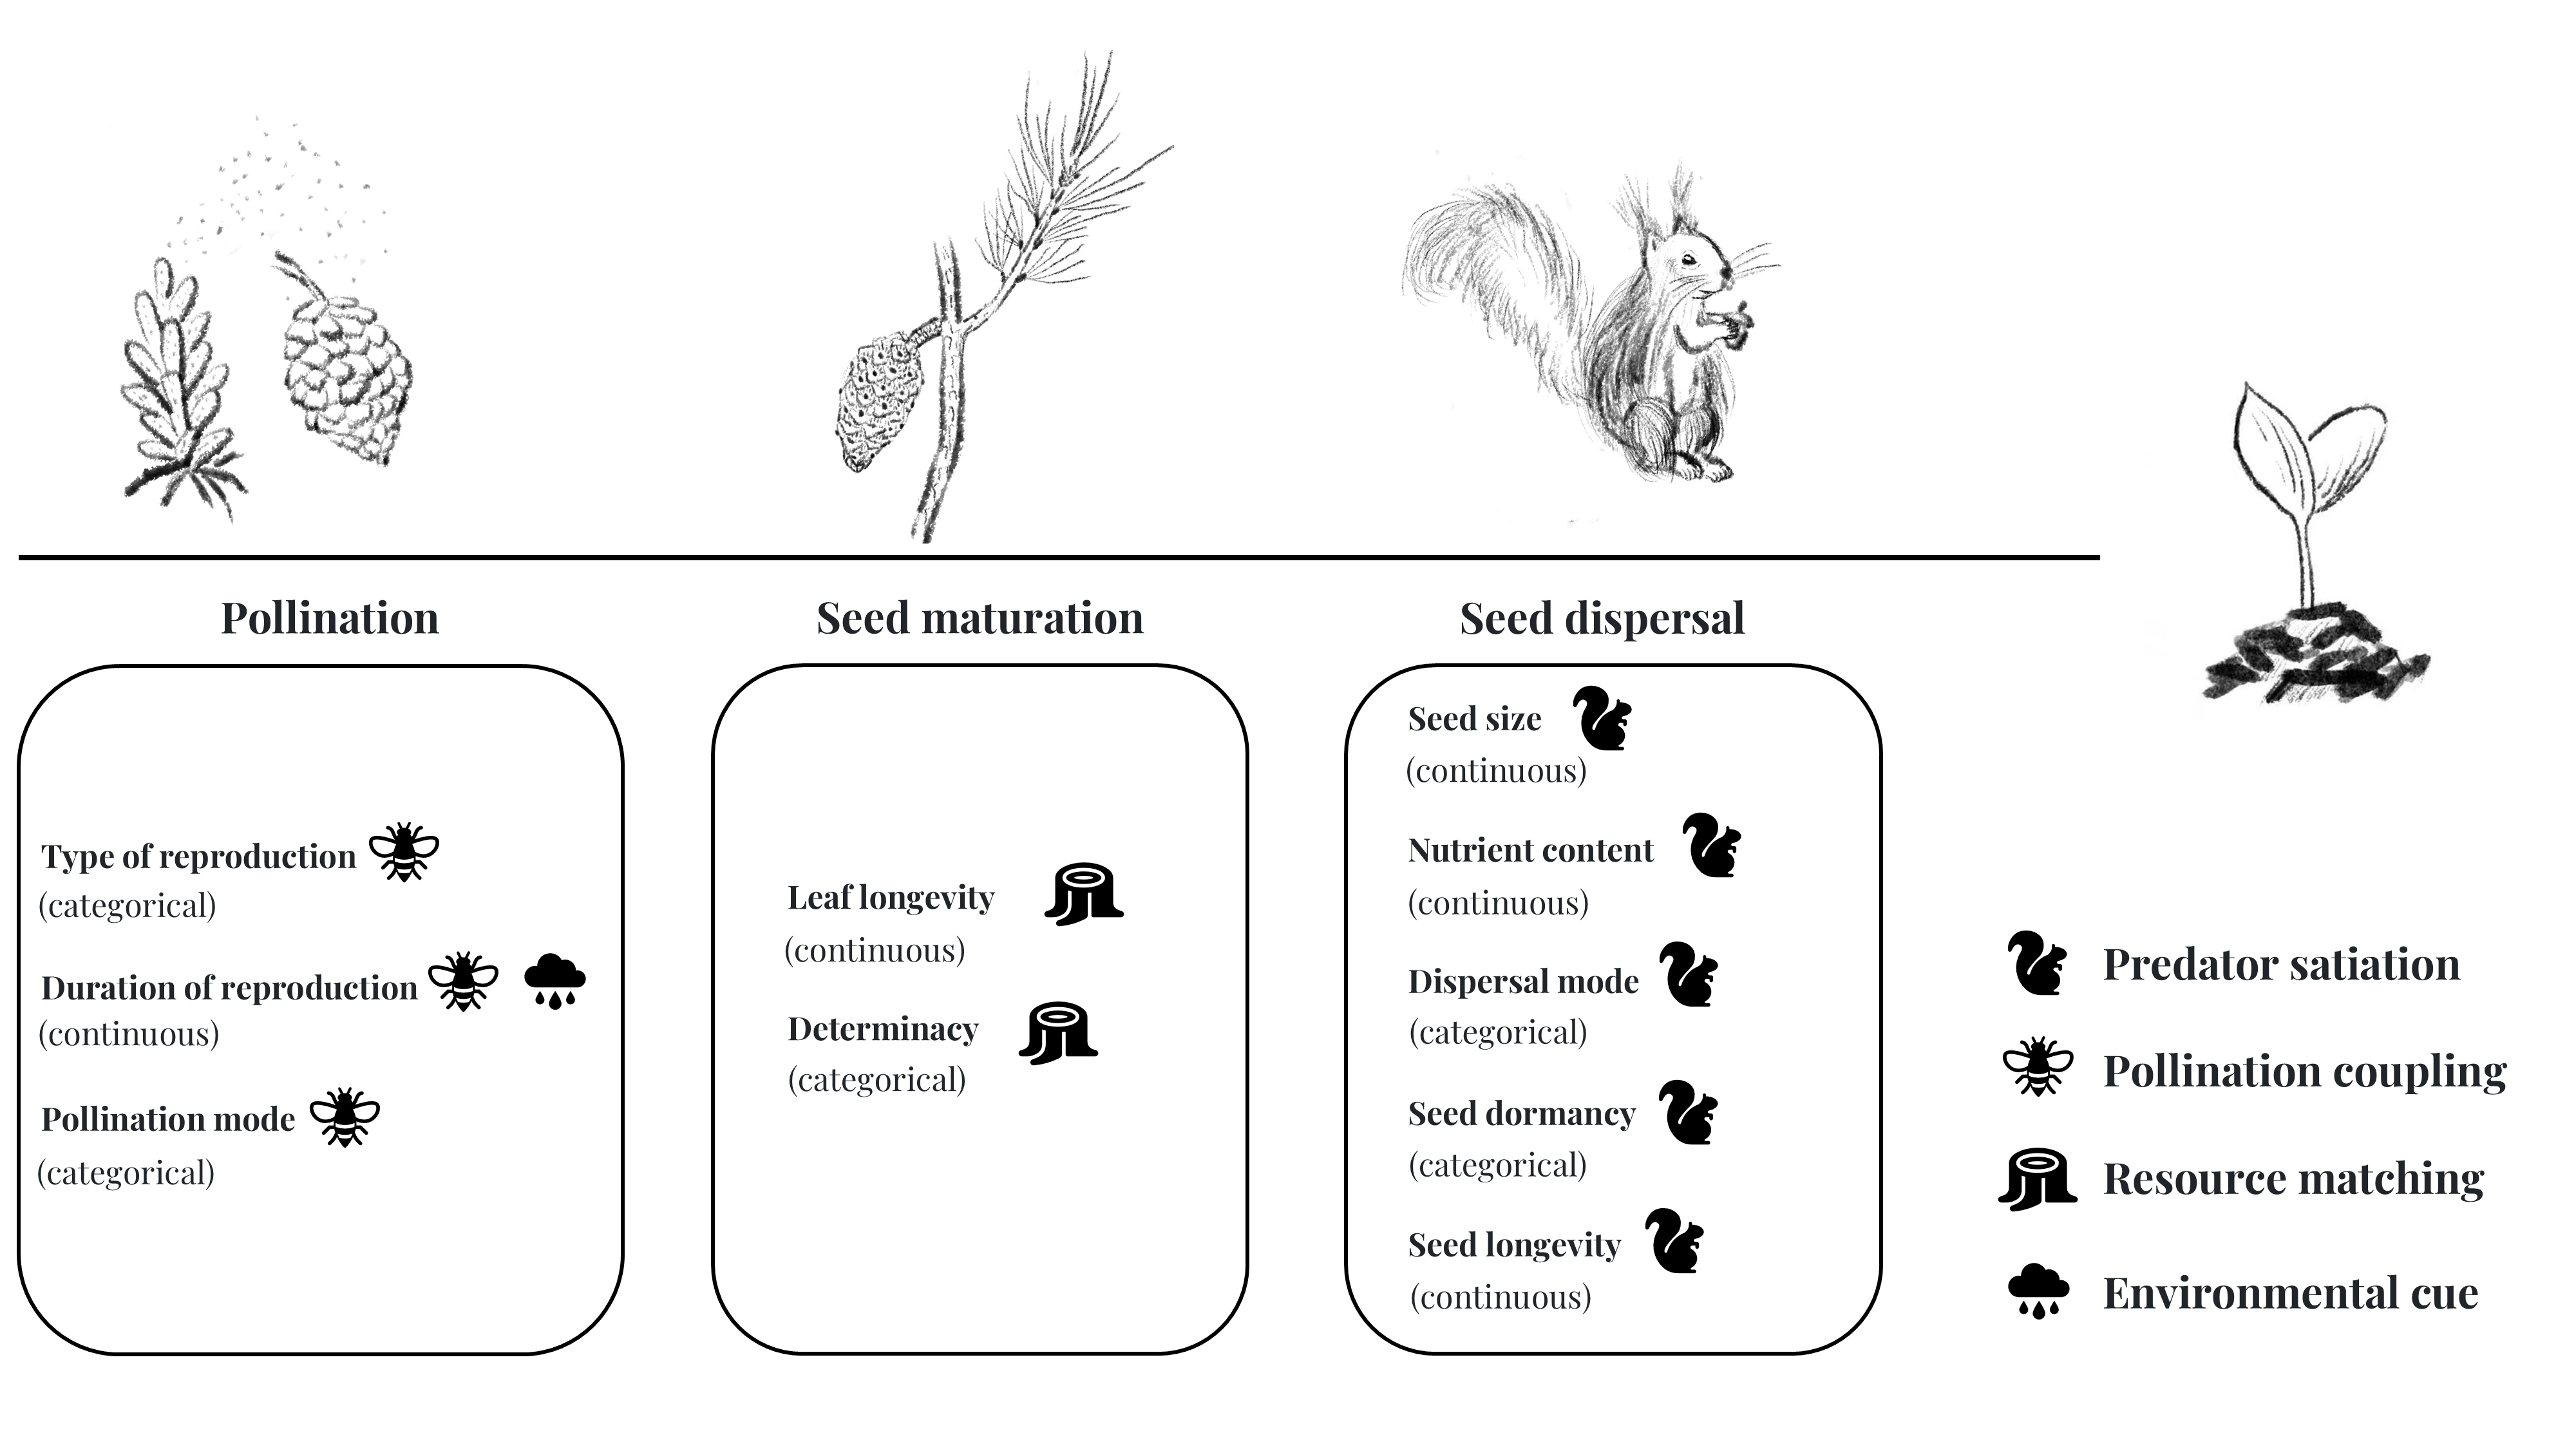
\includegraphics[width=1\linewidth]{conceptualChap1.png}
	\caption{Conceptual framework linking reproductive traits to the phenomenon of masting across critical stages of seed reproduction. The symbols indicate different hypotheses. I include the information on whether the traits are categorical or continuous below each trait.}
	\label{fig:conceptual1}
\end{figure}
\begin{figure}[htb]
	\centering
	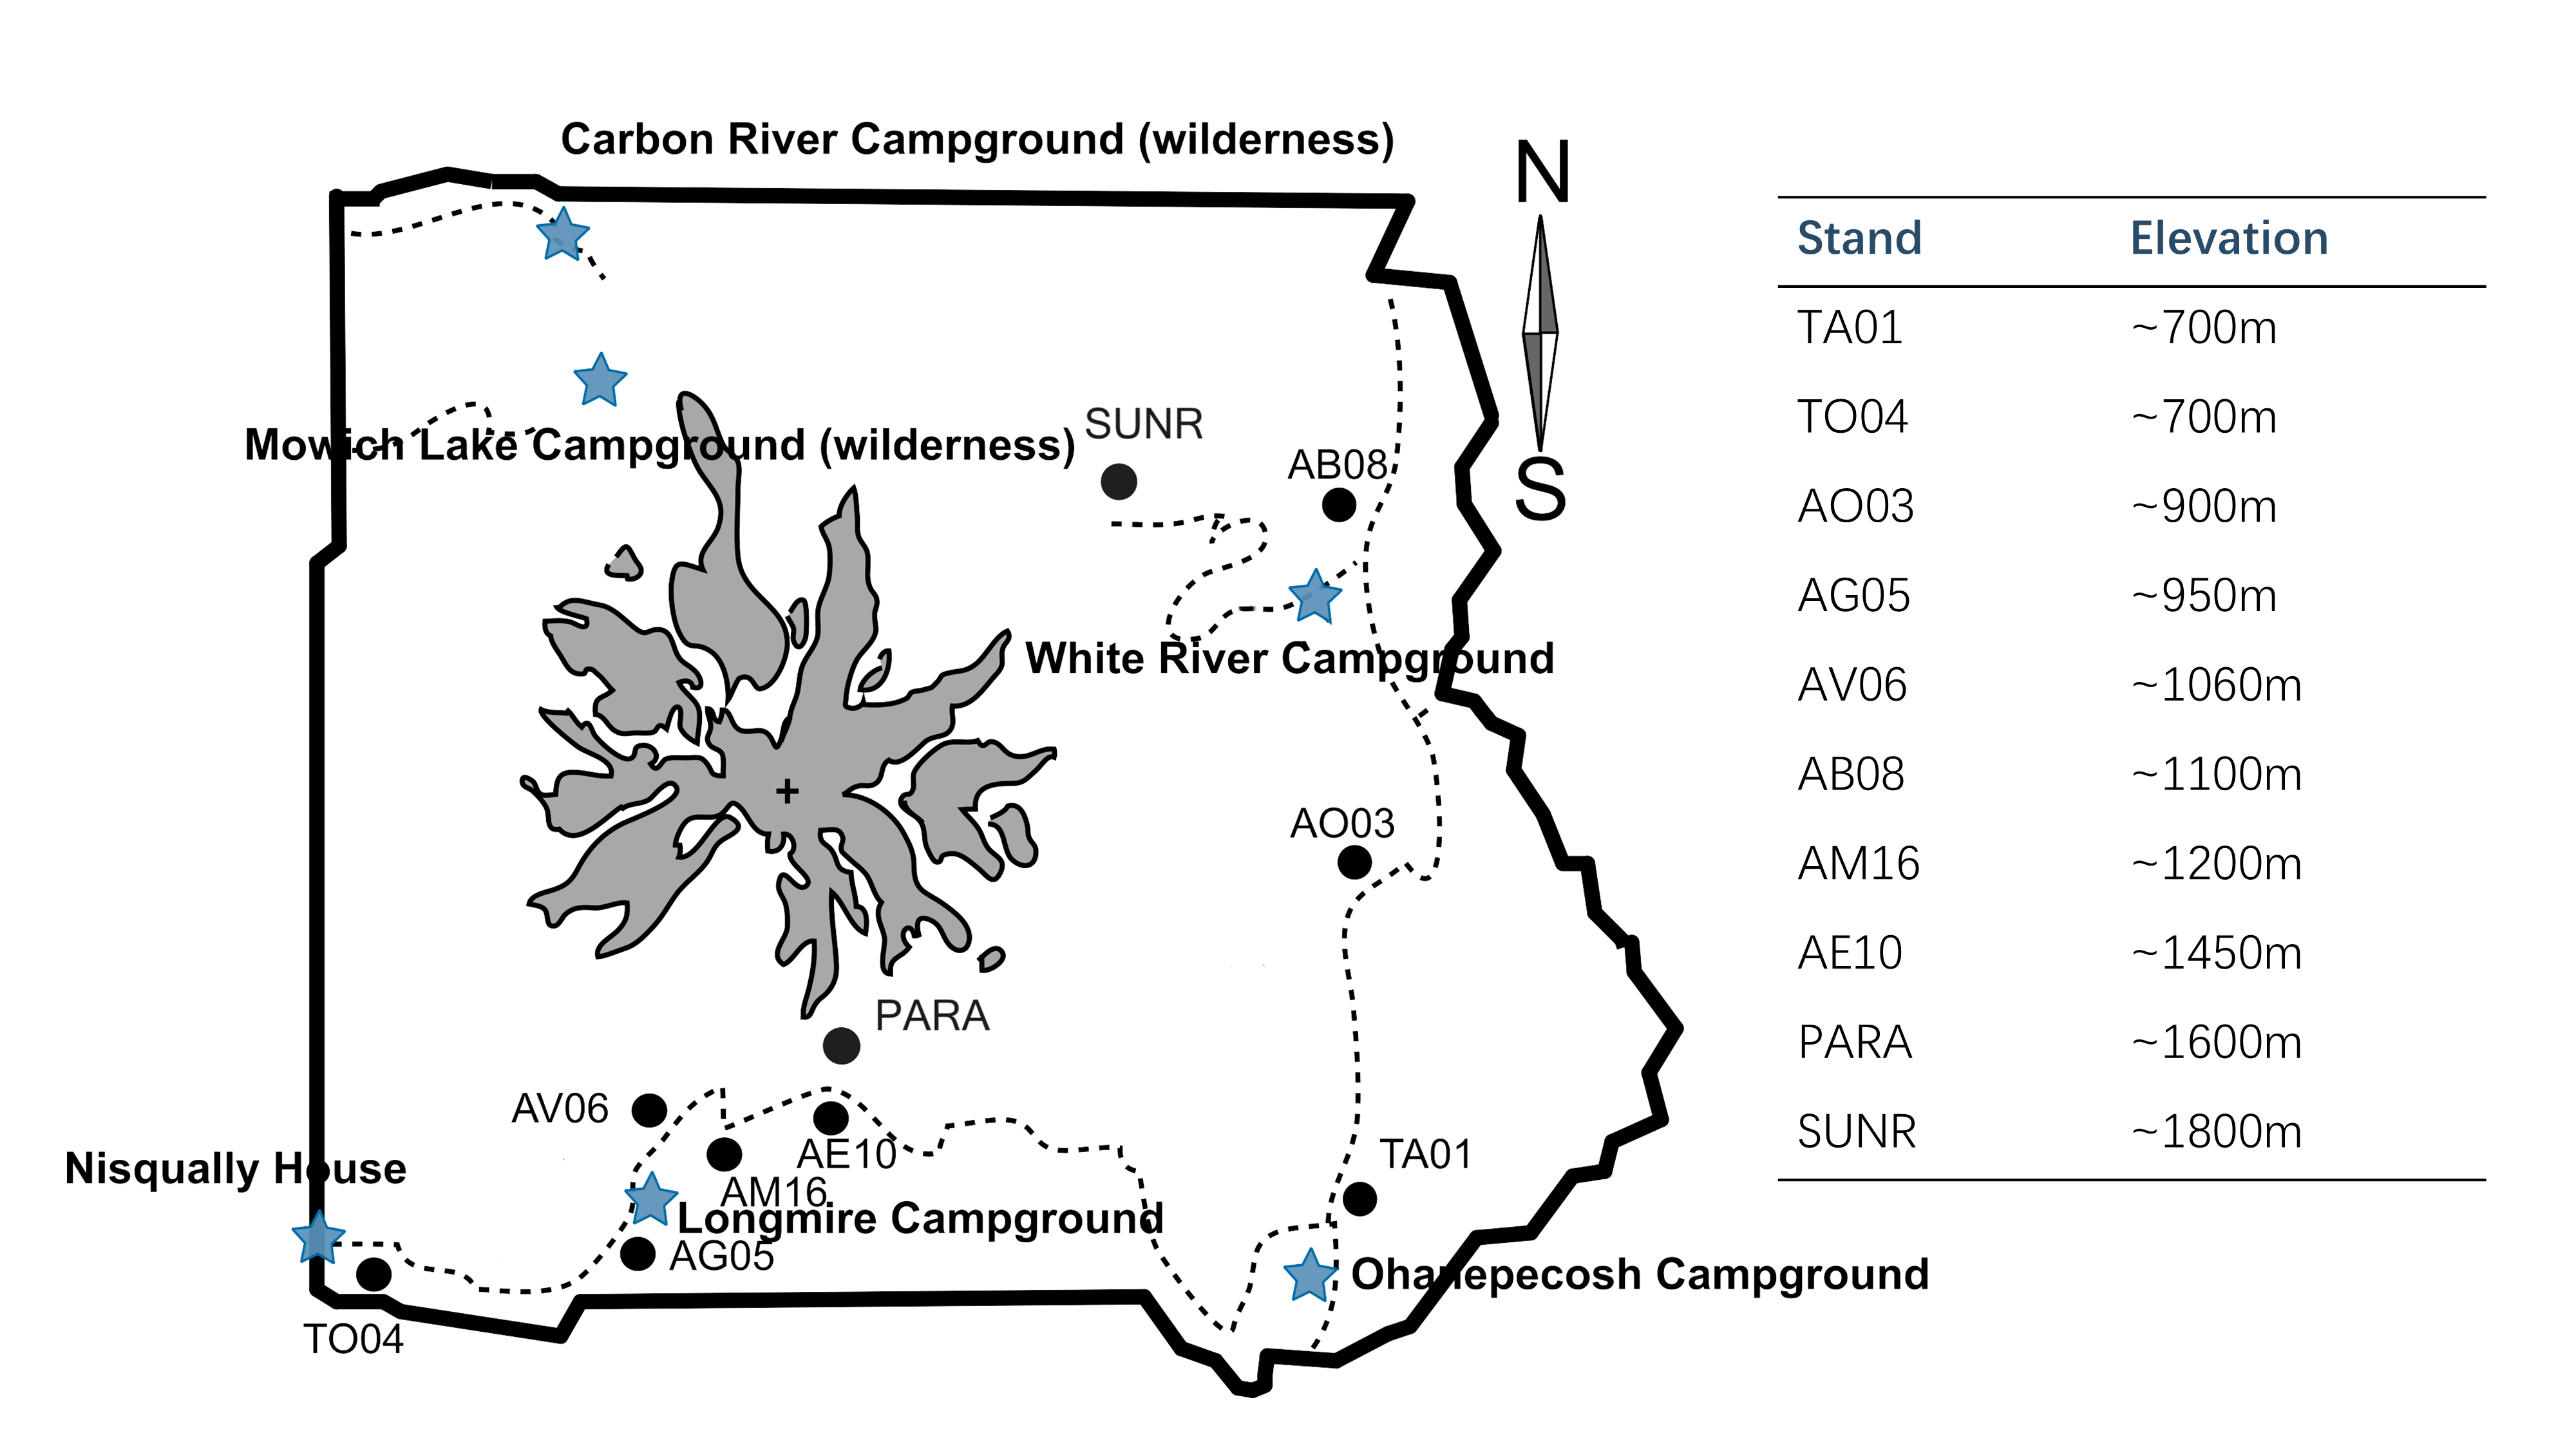
\includegraphics[width=1\linewidth]{rainierMap.png}
	\caption{A map of Mount Rainier with all the sampling stands for this study and the elevation of each stand. The black dots are the stands with their elevations shown in table at right (Blue starts are campgrounds).}
	\label{fig:sites}
\end{figure}
\begin{figure}[htb]
	\centering
	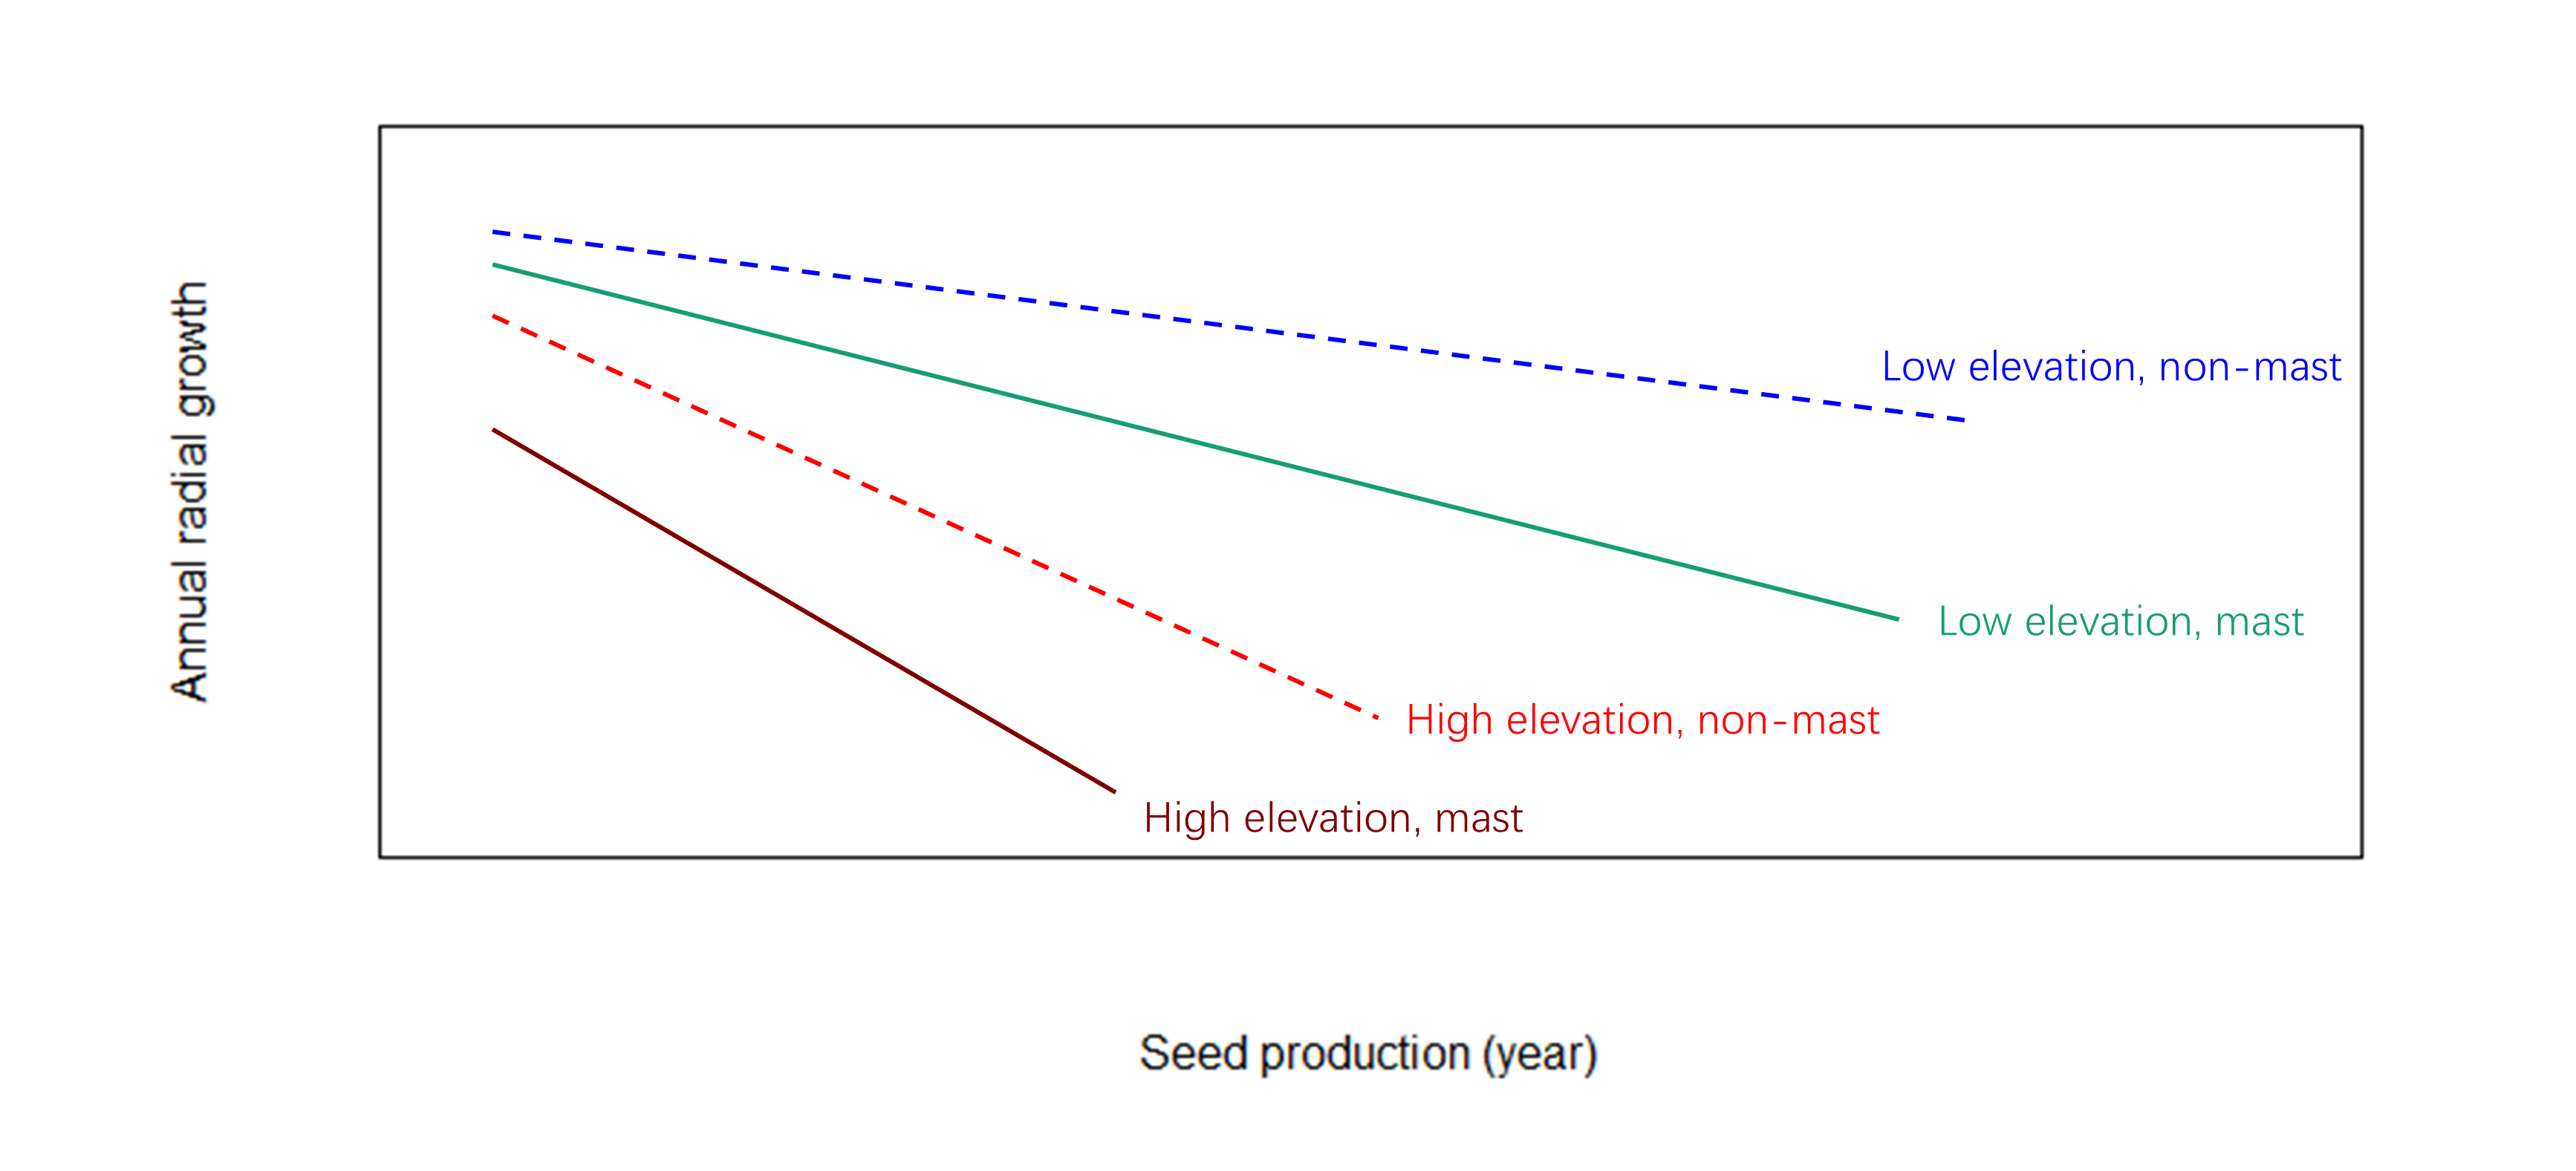
\includegraphics[width=1\linewidth]{conceptualFigureChap2.png}
	\caption{A conceptual figure showing the expected trend of growth-reproduction trade-off in masting years vs. non-masting years at different elevations. I predict that the trade-off is more pronounced in masting years compared to non-masting years in general and individuals at higher elevation stands would experience a higher trade-off.}
	\label{fig:conceptual2}
\end{figure}
\begin{figure}[htb]
	\centering
	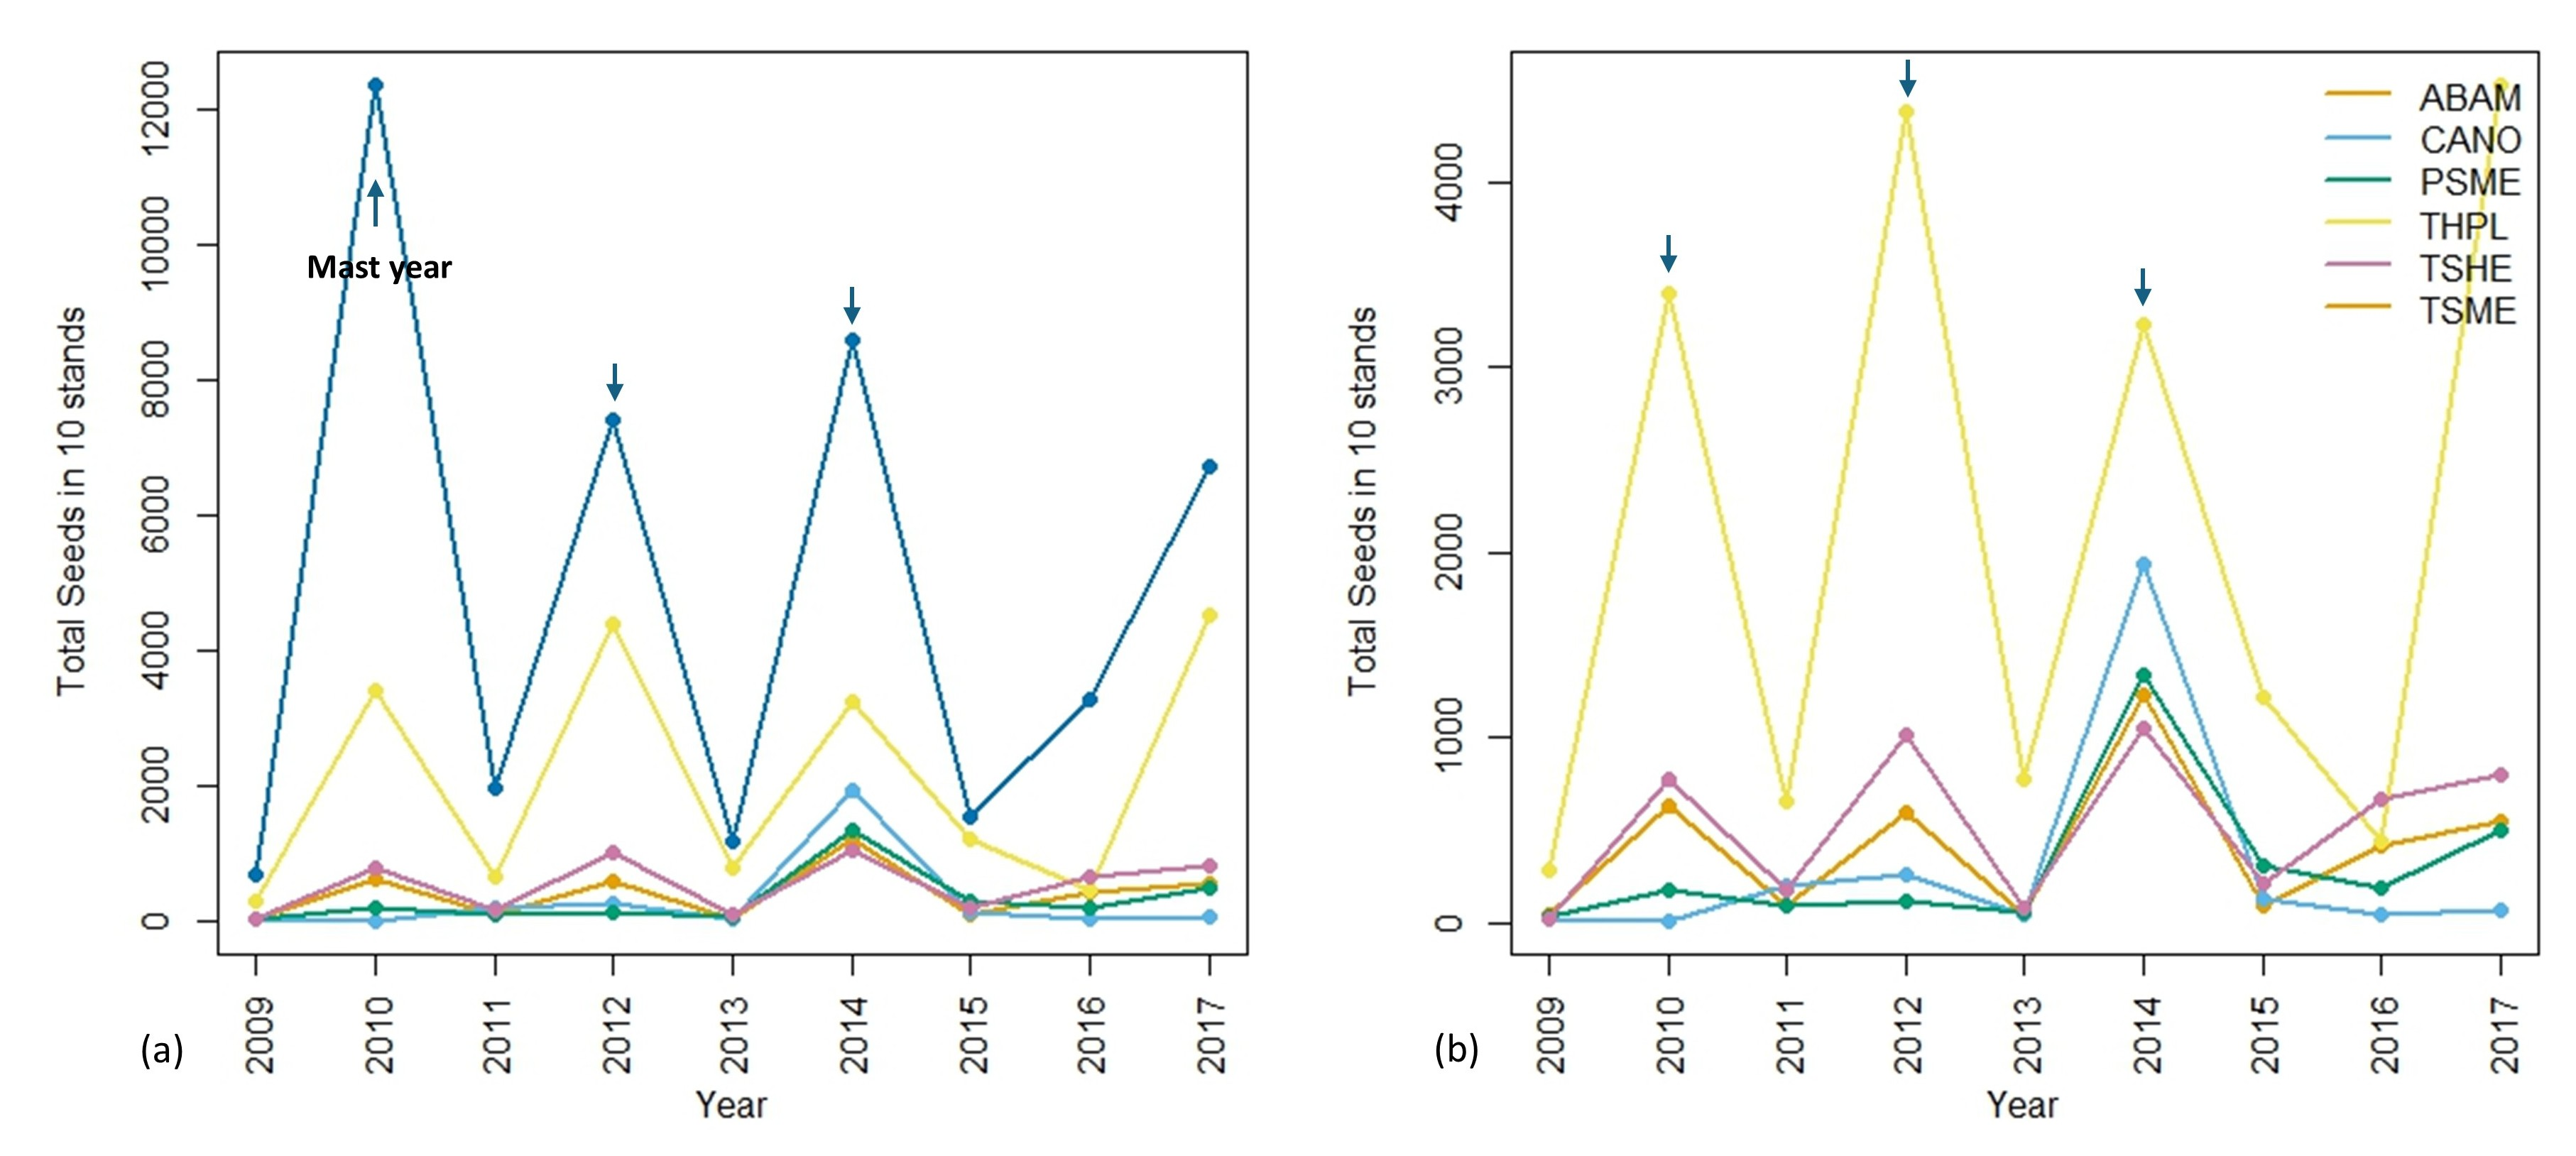
\includegraphics[width=1\linewidth]{Seed1.jpg} %emw17Apr2025: Can you confirm this really is the total? If so I would change (a) total seeds (sum of filled and empty seeds in all stands for each species  for each year), showing all six species of study. 
	\caption{Seed data across all 10 stands collected by seed traps from 2009-2017 at Mount Rainier. (a) total seeds (sum of filled and empty seeds) for all six species; (b) total seeds for only five species excluding TSHE in finer resolution with different y-axis scale. Short blue arrows indicate potential masting years. ABAM: \textit{Abies amabilis}, CANO:  \textit{Callitropsis nootkatensis}, PSME: \textit{Pseudotsuga menziesii}, THPL: \textit{Thuja plicata}, TSHE: \textit{Tsuga heterophylla}, TSME: \textit{Tsuga mertensiana}.}
	\label{fig:seed}
\end{figure}

\end{document}